\documentclass[12pt]{article}

\usepackage[T1]{fontenc} \usepackage[icelandic]{babel}
\usepackage{latexsym,amssymb,amsmath}
\usepackage{pgfplots}
\usepackage{float}
\usepackage[absolute,overlay]{textpos}
\newcounter{marknumber}
\pgfplotsset{
    error bars/every nth mark/.style={
        /pgfplots/error bars/draw error bar/.prefix code={
            \pgfmathtruncatemacro\marknumbercheck{mod(floor(\themarknumber/2),#1)}
            \ifnum\marknumbercheck=0
            \else
                \begin{scope}[opacity=0]
            \fi
        },
        /pgfplots/error bars/draw error bar/.append code={
            \ifnum\marknumbercheck=0
            \else
                \end{scope}
            \fi
            \stepcounter{marknumber}    
        }
    }
}
\usepackage{graphicx}
\graphicspath{ {./html/} }
\usepackage{hyperref, color}
\hypersetup{
    colorlinks=true,
    linktoc=all,
    linkcolor=blue,
}

\begin{document}


\centerline{\bf \Huge EÐL207G Verkefni 4 RCL}
\centerline{\bf Mikael Sævar Scheving Eggertsson, Torfi Þorgrímsson}

\centerline{\bf \large }

\tableofcontents
\newpage

\section{Inngangur}
Framkvæmdar voru tilraunir til að sjá hvernig spenna og straumur rafrása breytast þegar þéttir, spóla og/eða viðnám eru bætt inn. 
Notað er sveiflusjá til að mæla gildin. Í fyrri hlutanum finnum við hraða- og tímastuðul í RC- rás,
sú tilraun stóðst í samanburði við líkan. Seinni tilraun var leitað af horntíðni og dempunarstuðul
í RCL-rás, sú tilraun stóðst vel á einn hátt en hræðilega á annan. 
\section{Lýsingar}
\subsection{}

\setlength{\parindent}{0pt}

%3.1
\textbf{Stutt lýsing:}
Notuð er kassabylgja til að finna innra viðnám sveiflugjafans sem er mikilvægur partur að aðskilja frá heildarviðnámi rásarinar. 
Innra viðnámið fæst með því að tengja sveiflugjafan við viðnámsbox og stilla þannig að pólspennan er jöfn og hálf íspenna.
Út frá mælingu fæst að: $R_{innra}$ = 53ohm

\subsection{}
% 3.2

\begin{center}
    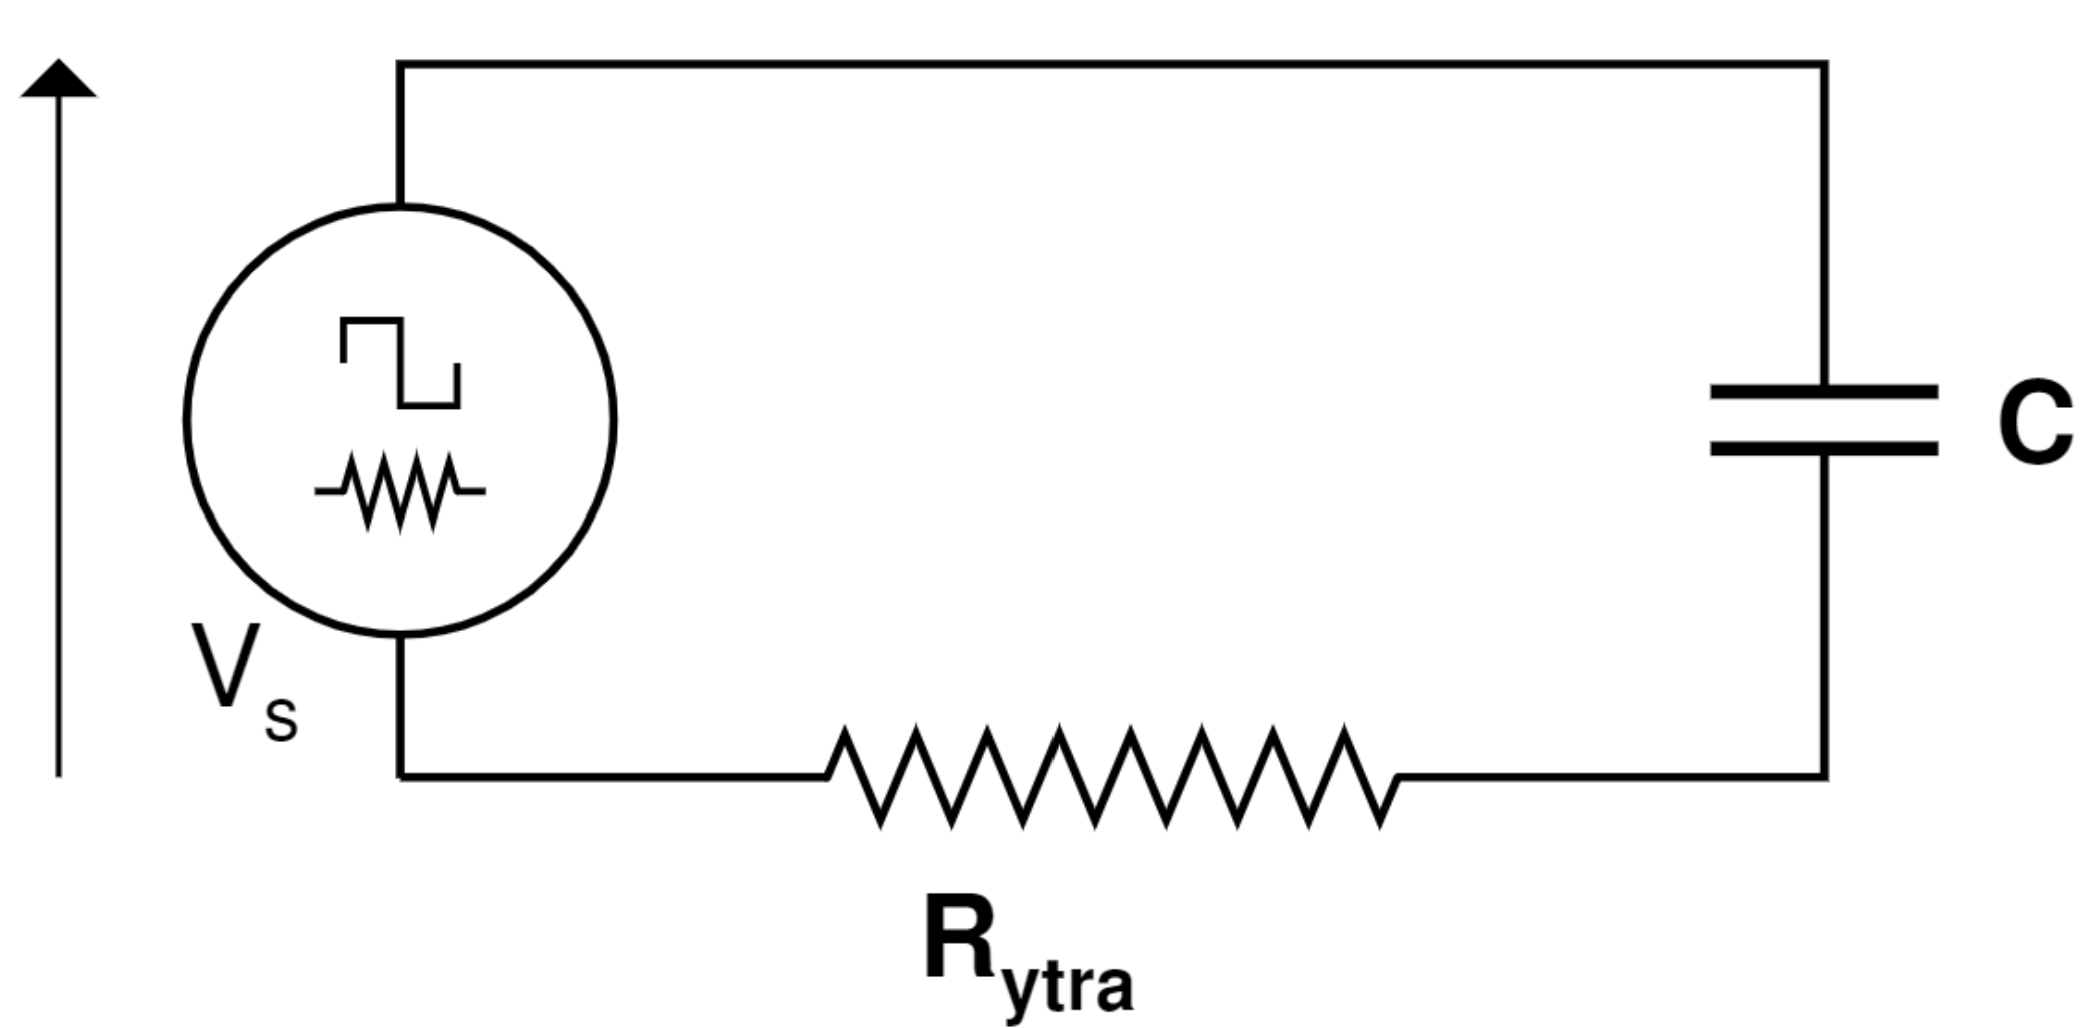
\includegraphics[scale=0.4]{mynd1}

Mynd 1
\end{center}

\bigskip

\textbf{Tákn notuð:}


$ \kappa $ er hraðastuðull


$ \tau $ er tímastuðull 


$ V $ er spenna 


$ V_R $ er spenna yfir ytra viðnám 


$ V_{R0}$ er hæsta spenna í bylgju 0 


$ R_{alls}$ er heildarviðnám rásarinnar 


$ C $ er rýmd þéttis 


\bigskip

\textbf{Stutt lýsing:}
Mynduð er RC-rás eins og á mynd 1 úr spennugjafa, þétti og stillanlegum viðnámskassa. Spennugjafinn er stilltur á kassabylgju með tíðnina 1kHz,
 gildið á þéttinum er þekkt sem 10nF og viðnámið er stillt á $ 5k \Omega$. Mæld eru 8 mismunandi gildi á tíma og spennu, niðurstöðurnar eru settar
  í spennu á tíma graf til að finna hraða- og tímastuðul.


\textbf{Jöfnur notaðar:}

\bigskip
$ \kappa = \dfrac{1}{R_{alls} *C}$ (1)
\bigskip


$ \tau = \dfrac{1}{\kappa}  $ (2)
\bigskip

$ \kappa = \dfrac{\ln{V_{R0}}-\ln{V_R}}{t}$ (3)
\bigskip


$ \Delta \kappa =  \dfrac{1}{tV_R}\Delta V_R + \dfrac{ln(V)-ln(V_R)} {t^2} \Delta t $ (4)

\bigskip



\textbf{Mæld gidli:}


\begin{table}[H]
    \begin{tabular}{|c|c|c|c|c|c|c|c|c|}
    \hline
    $V_R(t) [V]$  & 2.88 & 2.40 & 1.60 & 1.08 & 0.72 & 0.48 & 0.36 & 0.24  \\
    \hline
    t[$\mu s$] & 0 & 10 & 30 & 50 & 70 & 90 & 110 & 130  \\
    \hline
    \end{tabular}
\end{table}
 
\textbf{Úrvinnsla gagna:}

$ \kappa_0 = \dfrac{1}{RC} = 19.790$

\begin{table}[H]
    \begin{tabular}{|c|c|c|c|c|c|c|c|}
		t[$\mu s$] &10 & 30 & 50 & 70 & 90 & 110 & 130  \\
		\hline
		$ \kappa$ & 18.232 & 19.593 & 19.617 & 19.804 & 19.908 & 18.904 & 19.115 \\
		\hline
		$ \Delta \kappa$ & 1.182 & 529 & 3962 & 340 & 310 & 279 & 268\\
    \end{tabular}
\end{table}

%insert graf Vr af t
\begin{center}
    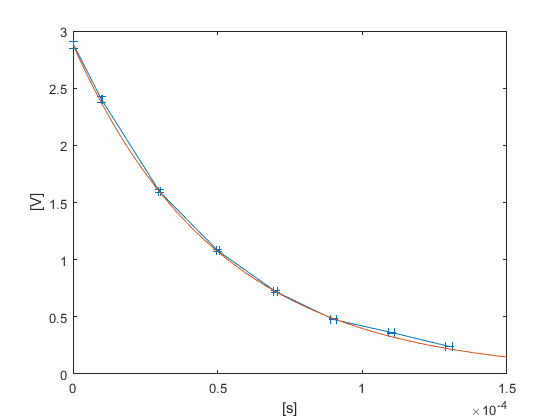
\includegraphics[scale=0.7]{data_01}

	Graf 1
\end{center}

\subsection{}
% 3.3

\begin{center}
    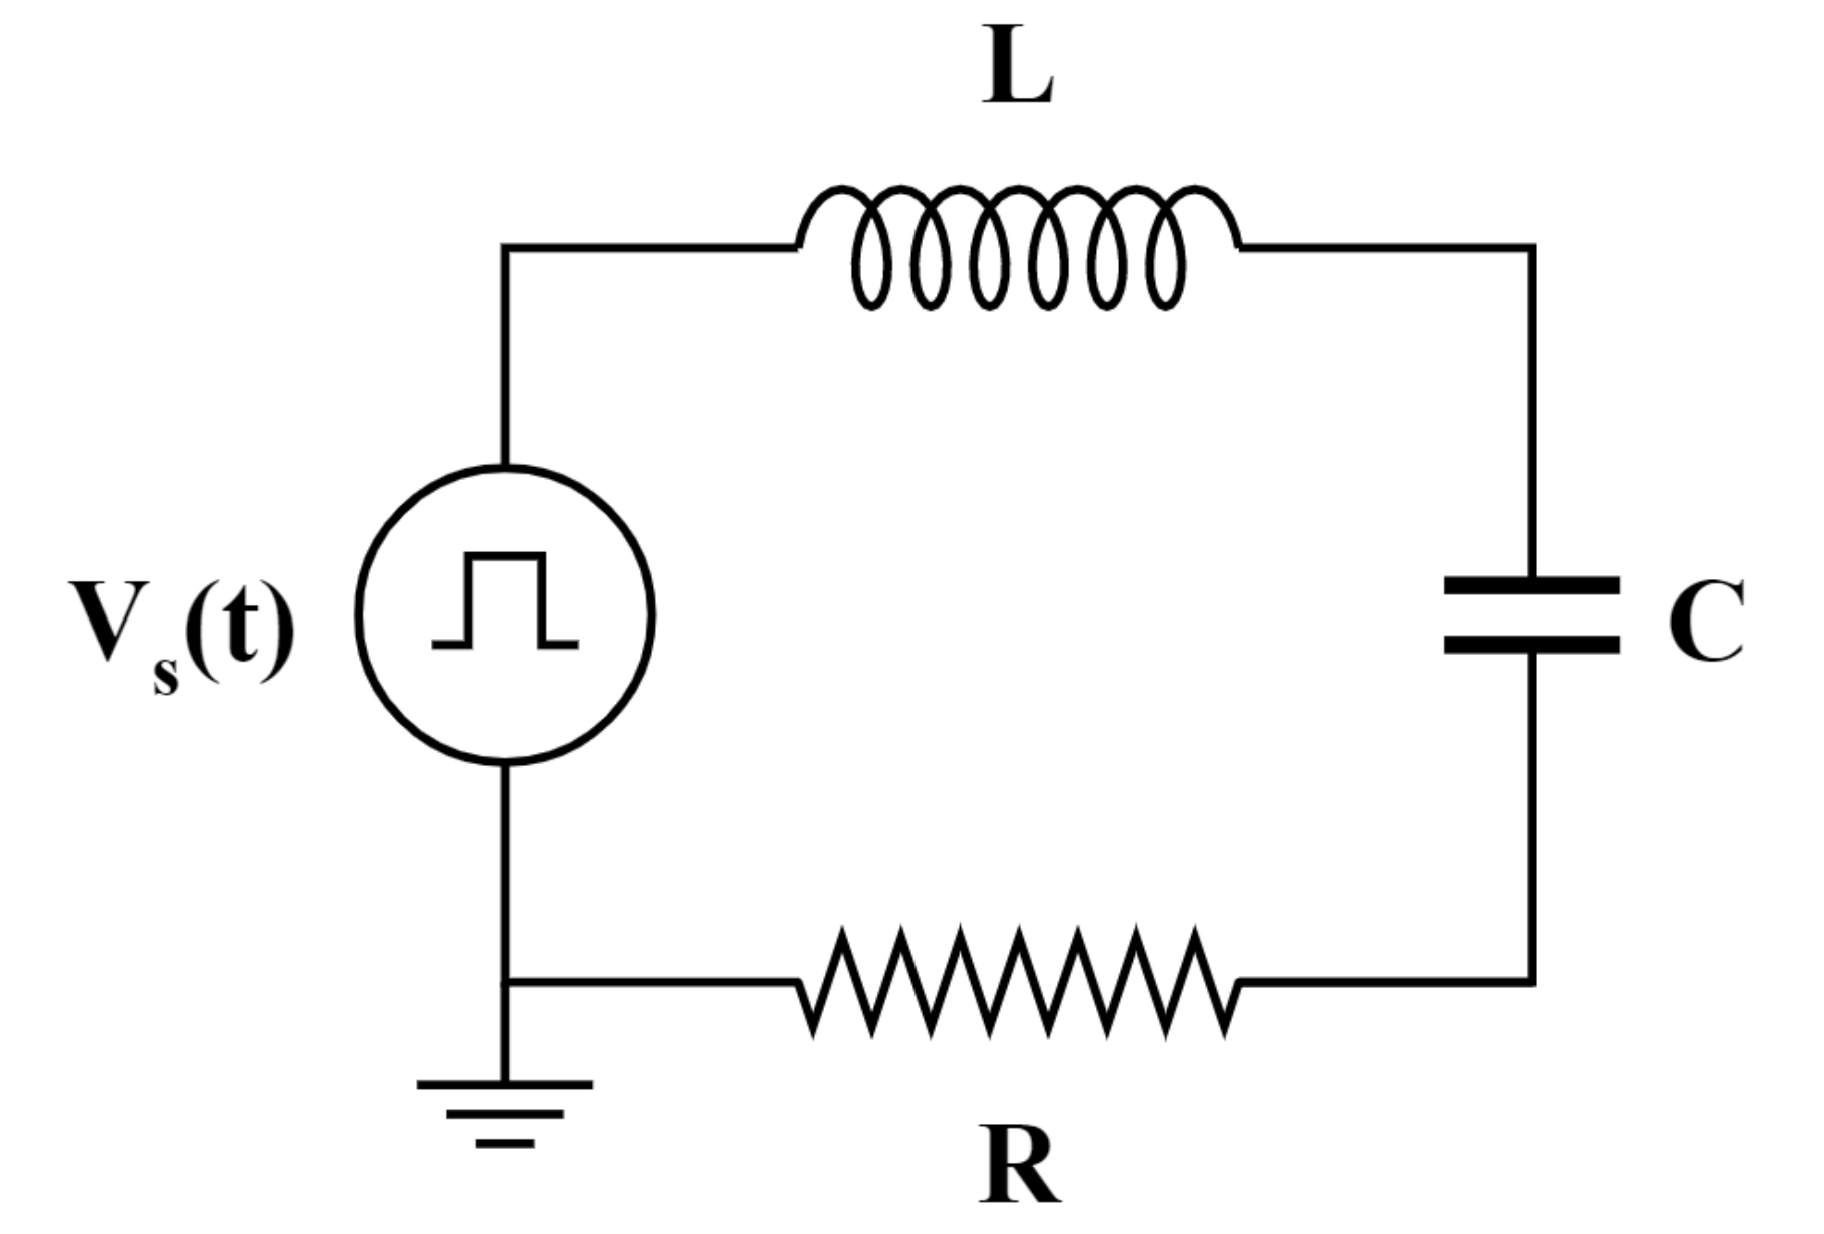
\includegraphics[scale=0.4]{mynd2}
    
    Mynd 2

\end{center}

\bigskip

\textbf{Tákn notuð:}


$ b$ er deyfingarstuðullinn


$ \omega$ er horntíðnin 


$ L $ er spanstuðull spólunar


$ R_m $ er viðnámsgildi markdeifingu


$ \phi $ er hliðrun bylgjunar




\bigskip

\textbf{Stutt lýsing:}
Búin til er RCL-rás eins og á mynd 2 með sveiflugjafa, þétti, spólu, og stillanlegum viðnámskassa. 
Spennugjafinn er stilltur á kassabylgju með tíðnina 1kHz,
þéttirinn er 10nF og spólan er 10mH, viðnámskassinn var stltur á $110 \Omega$. 
Mældir eru tindarnir og dalirnir á sveiflunum úr úrvinnslu á þeim
gögnum fást gildin fyrir $b$ og $\omega$.


\noindent{\textbf{Jöfnur notaðar:}}

\bigskip
$A\sin(\omega t + \phi)e^{-b t}$ (5)

\bigskip

$ \omega_0 = \sqrt{\frac{1}{LC}}$ (6)

\bigskip

$ b_0 = \dfrac{R}{2L}$ (7)

\bigskip
$ \omega_{e0}^2 = \omega_0^2-b_0^2 $ (8)

\bigskip

$ R_m^2 = \dfrac{4L}{C}$ (9)

\bigskip
$ n = -\dfrac{1}{4}+ \dfrac{t\omega _e}{2\pi} $ (10)

\bigskip
$\Delta \omega_e = \dfrac{\pi (4n+1)}{2t^2}\Delta t$

  
\bigskip
  \noindent{\textbf{Mæld gidli:}}

\begin{table}[H]
    \begin{tabular}{|c|c|c|c|c|c|c|c|c|}
    \hline
    $V_R(t) [V]$  & 0.576 & -0.432 & 0.328 & -2.40 & 0.176 & -0.128 & 0.096 & -0.072 \\
    \hline
    t[$\mu s$]    & 16.0 & 48.0 & 79.5 & 112.0 & 142.0 & 173.5 & 204.5 & 236.5 \\
    \hline
    \end{tabular}
\end{table}

\noindent{\textbf{Úrvinnsla gagna:}}

\subsubsection{}
Fyrst eru fundin hentug gildi fyrir $\omega, A$ og $b$. Það er gert með því að stilla $\omega_0=\sqrt{\frac{1}{LC}}$ 
og svo reikna út hin gildin út frá tvem mælipunktum. Svo er stungið falli sem lísir dempaðri sínus bylgju 
í fminsearch fallið í matlab með hentugu byrjunar gildin sem við fundum og út kemur:

\begin{table}[H]
    \begin{tabular}{|c|c|c|}
		$ A $ 	& $ \omega $ 	& $ b $ \\
		\hline
		0.6687 	& 9.7579e4		& 9.053e3 \\
    \end{tabular}
\end{table}


Og með þessum tölum getum við teiknað grænu línuna í grafi 2, sem passar mjög vel við mælingar okkar. Með fylgistuðul af 0.999974, Þó við höfum ekki óvissur fyrir þessi gildi.

Hinsvegar, við tökum eftir að við búumst við dempunarstuðul $b=\frac{R}{2L}=5500$, langt fyrir neðan mælda gildið $9053$. Augljóslega er raunveruleikinn mikill dempari.

\subsubsection{}

Næst er bláa línan, hún er breytingin á t með bylgju toppum, hún er bein, við búumst við að hún sker við y-ás við 1/4, sem hún gerir.

%insert graf n af t
\begin{center}
    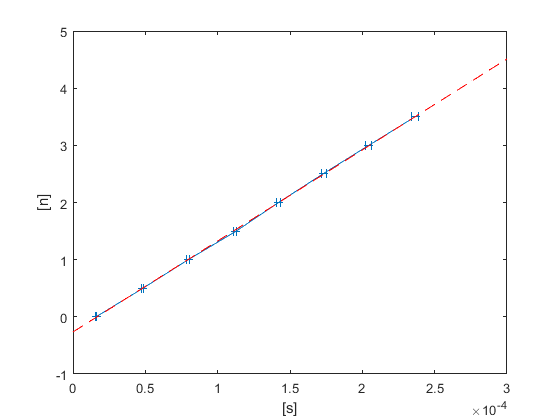
\includegraphics[scale=0.7]{data_03.png}
    
	Graf 2
\end{center}


Með þessu getum við reiknað $\omega_e$ með jöfnu (10)

Hinsvegar, við höfum líka jöfnu (8) til að reikna $\omega_e$, og þar af getum við notað bæði líkan gildin og þau mældu. Þar af fáum við:

$\omega_{e,\text{líkan}} = 99.849$
\qquad
$\omega_{e,\text{mæld}} = 97.224$

Hins-hinsvegar, höfum við ekki óvissu fyrir þessi gildi.

En fyrir jöfnu (10) er $\dfrac{\Delta \omega_e}{\omega_e} = \dfrac{\Delta t}{t} = 0.01$


\begin{table}[H]
    \begin{tabular}{|c|c|c|c|c|c|c|c|c|}
		$ \omega_e $ & 490.870 & 229.070 & 177.830 & 154.270 & 143.810 & 135.800 & 130.580 & 126.200  \\
		\hline
		$\Delta \omega_e$ &	4.908 & 2.290 & 1.778 & 1.542 & 1.438 & 1.358 & 1.305 & 1.262  \\
    \end{tabular}
\end{table}

Vá! Mikill munur og mikil dreyfing! 
Og fyrri gildin eru langt fyrir utan þau öll!

Ef við skoðum grafið, líkanið er hægri hliðrað á meðað við mæli punktana, þetta sést líka ef við notum ítrekari formúlu fyrir líkanið okkar og plúsum cos og fasta við jöfnu (5). 

Þannig að, kanski mínkar munurinn ef við hliðrum göngin okkar til hægri? Nei. Allar tölurnar minka en munurin er sá sami.

\section{Niðurstöður}

\subsection{}
Í tilraun 1 er ekkert líkan til að bera við, eins og er gert ráð fyrir að sú mæling sé með rétt gildi, 
en sá gildi var mikilvægt til að fá skýrari niðurstöður í hinum tveim liðunum.

\subsection{}
Frá grafinu sést að mældu gildi fyrir $ \kappa $ standast við líkanið nánast fullkomlega, þar til við endann þar
sem það skekkist aðeins og fellur utan skekkjumarka. Skekkjumörkin á y-ás minnka töluvert því lengra sem er 
komið inn á grafið af því að seinni liðurinn í jöfnunni er deildur með $ t^2 $. Því að $ \kappa $ og $ \tau $ eru
tengdir saman þá stenst $ \tau $ líka nánast fullkomlega við líkanið

\subsection{}
Gleymdist að skrá niður $ V_s $ meðan tilraun fór fram, en það hefur eingin áhrif á lokaniðurstöðuna. 
Reiknuð gildi út frá mælingum fyrir $\omega_0$ standast innan óvissumarka í samanburði við líkan. 
Hins vegar var mælda b ekki nálægt líkaninu með nánast tvöfalda stærð sem við vonuðumst eftir.
Afleiðingin á því var að $\omega_e$ endaði líka tvöfalt í samanburði við líkan, langt fyrir utan skekkjumarka. 




\end{document}